\documentclass[journal]{vgtc}                % final (journal style)
%\documentclass[review,journal]{vgtc}         % review (journal style)
%\documentclass[widereview]{vgtc}             % wide-spaced review
%\documentclass[preprint,journal]{vgtc}       % preprint (journal style)

%% Uncomment one of the lines above depending on where your paper is
%% in the conference process. ``review'' and ``widereview'' are for review
%% submission, ``preprint'' is for pre-publication, and the final version
%% doesn't use a specific qualifier.

%% Please use one of the ``review'' options in combination with the
%% assigned online id (see below) ONLY if your paper uses a double blind
%% review process. Some conferences, like IEEE Vis and InfoVis, have NOT
%% in the past.

%% Please note that the use of figures other than the optional teaser is not permitted on the first page
%% of the journal version.  Figures should begin on the second page and be
%% in CMYK or Grey scale format, otherwise, colour shifting may occur
%% during the printing process.  Papers submitted with figures other than the optional teaser on the
%% first page will be refused. Also, the teaser figure should only have the
%% width of the abstract as the template enforces it.

%% These few lines make a distinction between latex and pdflatex calls and they
%% bring in essential packages for graphics and font handling.
%% Note that due to the \DeclareGraphicsExtensions{} call it is no longer necessary
%% to provide the the path and extension of a graphics file:
%% 
\includegraphics{diamondrule} is completely sufficient.
%%
\ifpdf%                                % if we use pdflatex
  \pdfoutput=1\relax                   % create PDFs from pdfLaTeX
  \pdfcompresslevel=9                  % PDF Compression
  \pdfoptionpdfminorversion=7          % create PDF 1.7
  \ExecuteOptions{pdftex}
  \usepackage{graphicx}                % allow us to embed graphics files
  \DeclareGraphicsExtensions{.pdf,.PNG,.png,.jpg,.jpeg} % for pdflatex we expect .pdf, .png, or .jpg files
\else%                                 % else we use pure latex
  \ExecuteOptions{dvips}
  \usepackage{graphicx}                % allow us to embed graphics files
  \DeclareGraphicsExtensions{.eps}     % for pure latex we expect eps files
\fi%

%% it is recomended to use ``\autoref{sec:bla}'' instead of ``Fig.~\ref{sec:bla}''
\graphicspath{{figures/}{pictures/}{images/}{./}} % where to search for the images

\usepackage{microtype}                 % use micro-typography (slightly more compact, better to read)
\PassOptionsToPackage{warn}{textcomp}  % to address font issues with \textrightarrow
\usepackage{textcomp}                  % use better special symbols
\usepackage{mathptmx}                  % use matching math font
\usepackage{times}                     % we use Times as the main font
\renewcommand*\ttdefault{txtt}         % a nicer typewriter font
\usepackage{cite}                      % needed to automatically sort the references
\usepackage{tabu}                      % only used for the table example
\usepackage{booktabs}                  % only used for the table example
%% We encourage the use of mathptmx for consistent usage of times font
%% throughout the proceedings. However, if you encounter conflicts
%% with other math-related packages, you may want to disable it.

%% In preprint mode you may define your own headline.
%\preprinttext{To appear in IEEE Transactions on Visualization and Computer Graphics.}

%% If you are submitting a paper to a conference for review with a double
%% blind reviewing process, please replace the value ``0'' below with your
%% OnlineID. Otherwise, you may safely leave it at ``0''.
\onlineid{0}

%% declare the category of your paper, only shown in review mode
\vgtccategory{Research}
%% please declare the paper type of your paper to help reviewers, only shown in review mode
%% choices:
%% * algorithm/technique
%% * application/design study
%% * evaluation
%% * system
%% * theory/model
\vgtcpapertype{please specify}

%% Paper title.
\title{Oregon Traffic Accident Insights}

%% This is how authors are specified in the journal style

%% indicate IEEE Member or Student Member in form indicated below
\author{Nic Desilets, Alex Schultz, and Bungo Takahashi}
\authorfooter{
  %% insert punctuation at end of each item
  \item Nic Desilets is with Oregon State University. E-mail: desiletn@oregonstate.edu.
  \item Alex Schultz is with Oregon State University. E-mail: schulale@oregonstate.edu.
  \item Bungo Takahashi is with Oregon State University. E-mail: takahasb@oregonstate.edu.
}

%other entries to be set up for journal
\shortauthortitle{Desilets \MakeLowercase{\textit{et al.}}: Oregon Traffic Accident Insights}
%\shortauthortitle{Firstauthor \MakeLowercase{\textit{et al.}}: Paper Title}

%% Abstract section.
\abstract{
  This paper describes the problem that we addressing, why it is important, how visualizations can be effectively applied, potential users, and our general approach.
} % end of abstract

%% Keywords that describe your work. Will show as 'Index Terms' in journal
%% please capitalize first letter and insert punctuation after last keyword
\keywords{Traffic, accidents}

%% ACM Computing Classification System (CCS). 
%% See <http://www.acm.org/class/1998/> for details.
%% The ``\CCScat'' command takes four arguments.

\CCScatlist{ % not used in journal version
  \CCScat{K.6.1}{Management of Computing and Information Systems}%
  {Project and People Management}{Life Cycle};
  \CCScat{K.7.m}{The Computing Profession}{Miscellaneous}{Ethics}
}

%% Uncomment below to include a teaser figure.
\teaser{
  \centering
  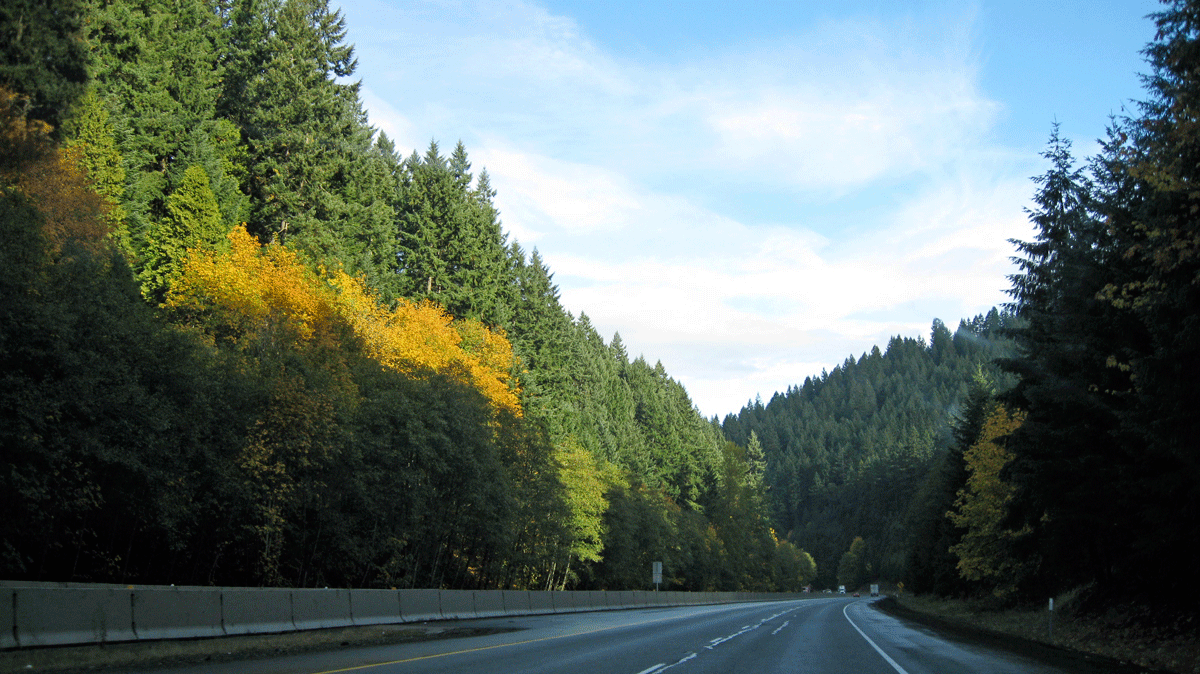
\includegraphics[width=\linewidth]{highway}
  \caption{Interstate 5 on the way to Portland, Oregon.}
  \label{fig:teaser}
}

%% Uncomment below to disable the manuscript note
%\renewcommand{\manuscriptnotetxt}{}

%% Copyright space is enabled by default as required by guidelines.
%% It is disabled by the 'review' option or via the following command:
% \nocopyrightspace

\vgtcinsertpkg

%%%%%%%%%%%%%%%%%%%%%%%%%%%%%%%%%%%%%%%%%%%%%%%%%%%%%%%%%%%%%%%%
%%%%%%%%%%%%%%%%%%%%%% START OF THE PAPER %%%%%%%%%%%%%%%%%%%%%%
%%%%%%%%%%%%%%%%%%%%%%%%%%%%%%%%%%%%%%%%%%%%%%%%%%%%%%%%%%%%%%%%%

\begin{document}

%% The ``\maketitle'' command must be the first command after the
%% ``\begin{document}'' command. It prepares and prints the title block.

%% the only exception to this rule is the \firstsection command
\firstsection{Introduction}

\maketitle

%% \section{Introduction} %for journal use above \firstsection{..} instead
Traffic accidents happen to a certain extent every year, and the number of fatal accidents in Oregon has been increasing. 
There are detailed reports on traffic accidents online; however, those reports include only numbers and not easy to see what correlations exist among the data. 
Therefore, we would like to visualize and organize the data in order to make it easier to see correlations between variables.
Hopefully this will lead to finding insights and solutions to help decrease the number of accidents. 

It is important that the problem needs to be addressed with a visualization because it’s easy to get lost in black and white statistics. 
It is difficult for a person to identify trends just by looking at thousands and thousands of rows of raw data each with many columns. 
Transforming this raw data into easy to digest visualizations will allow people to more easily recognize and address any trends hidden inside all the numbers. 
Potential users could range from the average person interested in traffic statistics to ODOT crew members and law enforcement members interested in evaluating effectiveness of certain policies aimed at reducing traffic accidents. 

Our approach is going to be to first process the data that we have gathered and put it into a SQL database so that we can more easily query the data for information that we’re interested in. 
From there, with the assistance of a user guide that is associated with our data set we will be able to identify trends within the data such as vehicular accidents per capita by county, amount of accidents resulting from drunk driving over time, and so on. 
Once we have identified the trends that we are interested in we will then develop a user interface containing visualizations of these trends so that people can interact with and understand them.

\section{Visualization Tasks}

Questions that we will address with the visualization are the following:
\begin{itemize}
  \item How many accidents happened depending on vehicles (car, motorcycles etc.).
  \item How many people were injured or killed in the accidents.
  \item What are the demographics of those involved in accidents (in terms of age, sex, residence).
  \item What caused the accidents (such as speed, road condition, light condition etc. ).
  \item Amount of accidents caused by drunk driving over time (or other intoxicants).
  \item Amount of accidents per capita over time (e.g. are accidents increasing or decreasing?).
\end{itemize}

\section{Data Source}

Our primary data source is going to be the National Highway Traffic Safety Administration (NHTSA). 
They have an FTP server hosting very detailed accident data ranging from 1976-2015. 
For our purposes we will only be looking at the past five to six years, partially because of inconsistencies within the data by year. 
Data from 2010 and on can be easily compared against each other while data before 2010 is setup differently and will be more difficult to compare. 
Additionally, we may be able to leverage ODOT accident data to supplement the data coming from the NHTSA.

\section{Data Organization}

We will be organizing our data into three entities. 
\begin{itemize}
  \item Vehicle Crash: datetime, location, cause, fatalities, conditions.
  \item Person: personal info, intoxicants involved, role in vehicle crash 
  \item Vehicle: make, model, year, status, issues, type
\end{itemize}

The relationships between these three entities are described below.
\begin{itemize}
  \item Fatal/Injury vehicle crash to person: 1 mandatory to many optional
  \item Person to Vehicle: 1 mandatory to 1 mandatory
  \item Fatal/Injury vehicle crash to Vehicle: 1 mandatory to many optional
\end{itemize}

\section{Implementation of ER Diagrams}

Figure 2 shows the Entity-Relationship diagram detailing the relationships between our stored entities.
We will be translating the ER diagrams into a schema for MySQL.
Once the data is loaded into the MySQL database the application used to show the data will be able to query the necessary data.

\begin{figure}[tb]
  \centering % avoid the use of \begin{center}...\end{center} and use \centering instead (more compact)
  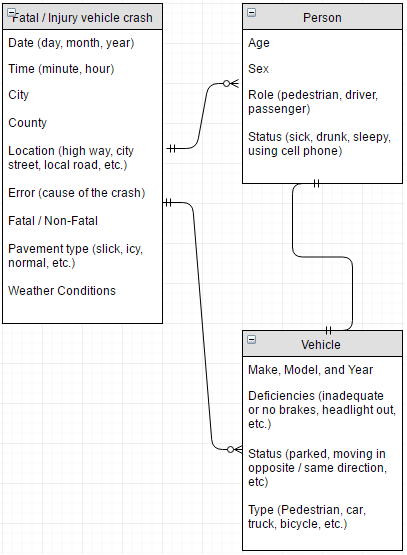
\includegraphics[width=\columnwidth]{entityrelationship}
  \caption{Entity-Relation diagram showing the relationships between vehicle crashes, people, and vehicles.}
  \label{fig:sample}
\end{figure}

\section{Design of Visualization Interface}

The primary component of the interface is going to be the map which shows accidents represented as a heat map. 
The data points used for the map will depend on what filters are set (e.g. number of all crashes, specific types of crashes, etc.).
There will be a slider that can be used to adjust what year is shown for the data (e.g. all accidents, accidents in 2015, accidents in 2014, etc.). 
Additionally, a legend will complement the map figure to help describe the elements show on the map. 
For example, if a heat map is used, the legend could be used to map colors to accident values.
Figure 3 details a mockup of our user interface. 

\begin{figure}[tb]
  \centering % avoid the use of \begin{center}...\end{center} and use \centering instead (more compact)
  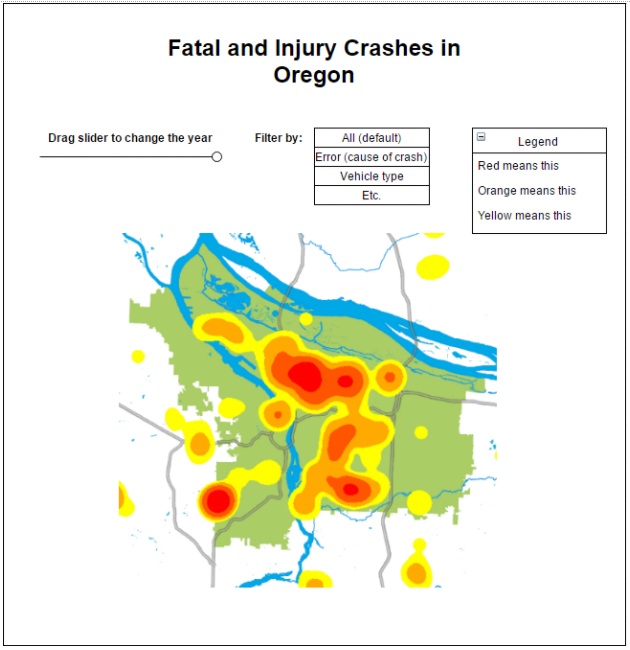
\includegraphics[width=\columnwidth]{interface}
  \caption{Mockup of our proposed user interface for displaying data.}
  \label{fig:sample}
\end{figure}

%% if specified like this the section will be committed in review mode
\acknowledgments{
  None.
}

%\bibliographystyle{abbrv}
\bibliographystyle{abbrv-doi}
%\bibliographystyle{abbrv-doi-narrow}
%\bibliographystyle{abbrv-doi-hyperref}
%\bibliographystyle{abbrv-doi-hyperref-narrow}

\bibliography{template}
\end{document}

